\hypertarget{component}{}\section{HSA Topology and Component
}\label{topology}
The HSA platform topology requirement is described in the SAR
document. The SAR document also depicts possible complex topologies
and potential data-structure associations to represent topology
hierarchy.  As a part of the HSA core base API functionality, the
user may query information about the HSA system to gather details
such as the number of host compute units and different HSA
Components on the system with local access to a set of memory
resources attached to the node's memory controller and appropriate
HSA-compliant access attributes. This information could be utilized
by the user in different ways including decisions on where to
execute a particular user task. 

Platform topology is represented as a table in the HSA runtime
implementation. See SAR section on \textbf{Requirement: HSA Platform
Topology Discovery} for description on the potential structure of
this table. There are five elements to the topology information:
agents, caches, physical memory, and when applicable, Translation
Lookaside Buffer (TLB) and I/O interconnects. HSA platform can have
a complex structure with multiple nodes and each node with multiple
components and physical memories. For its user, the core runtime
encapsulates the topology information. The topology table is
internal to runtime. The runtime defines a structure,
\dbtt{hsa\_platform\_t} that represents properties such as the
clock frequency that are common across the platform and also links
to various elements in the topology table (see Figure
\ref{fig:tablemap} ).
It is defined as follows:

\input{STRhsa_platform}

\begin{figure}
  \centering
  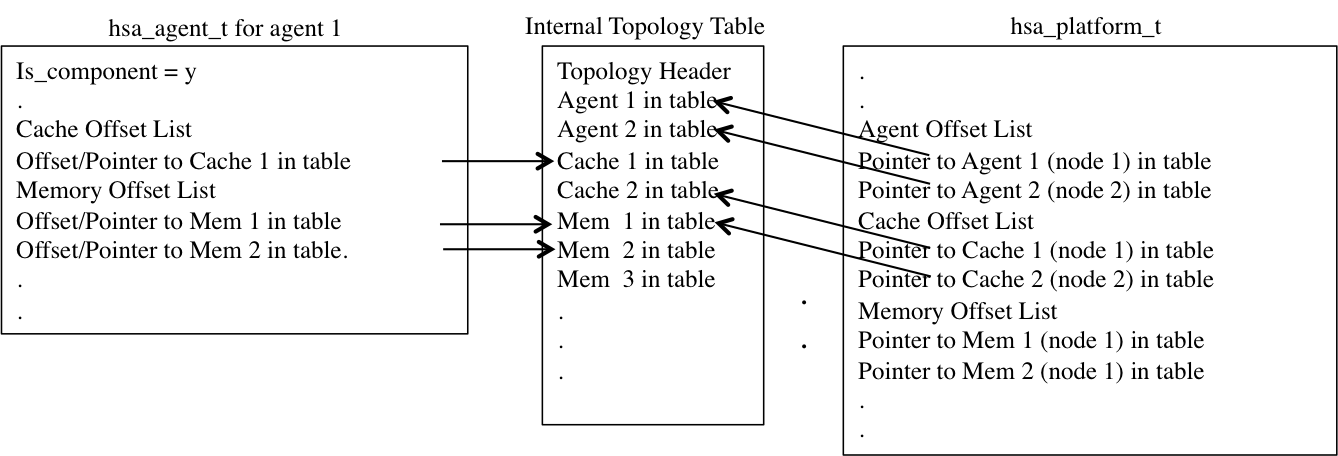
\includegraphics[width=0.5\textwidth] {maptoagent}
  \centering
  \caption{Mapping of Agent and Platform Structures to Topology
Table}
  \label{fig:tablemap}
\end{figure}

When no information is available about a particular element, the
corresponding {\itshape number\_ \textless element \textgreater s}
field is set to zero by the runtime in the platform structure.
Platform structure maps to the agents, cache and physical memory,
etc.\, in the topology table for all the nodes in the platform.

The core runtime defines the following structure to represent cache:

\input{STRhsa_cache_descriptor}

The structure holds associativity, cache size, cache line size for
all levels of cache and the inclusivity property for all but the
last level. Each cache in the HSA system has a unique cache ID
identifying it. 

The structure representing TLB is very similar to the one for cache,
with associativity, levels and inclusivity. It is defined as follows:

\input{STRhsa_tlb_descriptor}

The memory descriptor structure represents a physical memory block
or region and includes elements to provide provide bandwidth, interleave
characteristics and latency for accessing memory. Implementations
may choose not to provide memory bandwidth or latency information.
The memory descriptor structure is defined as follows:

\input{STRhsa_memory_descriptor} 

The structure: 
\input{STRhsa_segment} 
can represent any combination of of the 7 HSA segments, a single
bit for each segment. 

The HSA Agent data structure represents an HSA component when the
{\itshape is\_component} field in the agent structure is set to a 1.
The structure contains elements that describe its properties. Each
component has access to coherent global memory (the HSA global
segment, and as per the requirement defined in SAR, has access to
other segments as well). 

The structure of the HSA agent/component is defined as follows:

%\input{ENUagent_type}
\input{STRhsa_component}
